\documentclass[12pt,a4paper]{report}

\usepackage{array}
\usepackage{makecell}
\usepackage{microtype}
\newcolumntype{L}[1]{>{\raggedright\let\newline\\\arraybackslash\hspace{0pt}}m{#1}}
\newcolumntype{C}[1]{>{\centering\let\newline\\\arraybackslash\hspace{0pt}}m{#1}}
\newcolumntype{R}[1]{>{\raggedleft\let\newline\\\arraybackslash\hspace{0pt}}m{#1}}

\usepackage{mathptmx}
\usepackage{graphicx} % Required for inserting images
\graphicspath{{img/}}
\usepackage{multirow}
\usepackage{caption}
\usepackage{longtable}

\usepackage{geometry}
\geometry{
	top=4cm,
	right=3cm,
	left=4cm,
	bottom=3cm,	
}

\usepackage{pdflscape}
\usepackage{tabularray}
\usepackage[table]{xcolor}
\usepackage{setspace}
\onehalfspacing
  
\renewcommand{\thechapter}{\centering \Roman{chapter}}
\renewcommand{\thesection}{\arabic{chapter}.\arabic{section}}

\def\contentsname{DAFTAR ISI}
\renewcommand\bibname{DAFTAR PUSTAKA}
\def\chaptername{BAB}

\usepackage{titlesec}
\titleformat{\chapter}[display]{\normalfont\bfseries\centering}{\MakeUppercase{\chaptertitlename}~\thechapter}{0pt}{}
\titlespacing*{\chapter}{0pt}{-2pt}{16pt}

\renewcommand{\arraystretch}{1.5}

\renewcommand\thechapter{\Roman{chapter}}
\renewcommand\thesection{\arabic{section}}
\def\thesection{\arabic{chapter}.\arabic{section}}
\def\thetable{\arabic{table}}

\titleformat{\section}[block]{\bf\normalsize}{\thesection}{0.6em}{}
\titlespacing*{\section}{0pt}{5pt}{0pt}
\titleformat{\subsection}[block]{\bf\normalsize}{\thesubsection}{0.6em}{}
\titlespacing*{\subsection}{0pt}{5pt}{0pt}

\usepackage{setspace}
%\singlespacing
\onehalfspacing
%\doublespacing
%\setstretch{1.1}
\renewcommand{\tablename}{Tabel}
\renewcommand{\figurename}{Gambar}
\renewcommand{\thefigure}{\thesection.\arabic{figure}}
\renewcommand{\thetable}{\thesection.\arabic{table}}
\usepackage[breaklinks]{hyperref}
\renewcommand{\listfigurename}{DAFTAR GAMBAR}
\renewcommand{\listtablename}{DAFTAR TABEL}

\hyphenation{me-la-in-kan}

\newcommand{\nim}{1990343064}							% NIM Mahasiswa 
\newcommand{\mahasiswa}{Ahlul Mukhramin}	% Nama Mahasiswa
\newcommand{\judulId}{Rancang Bangun Game Multiplayer Online First Person Shooter(FPS) 3D Menggunakan Photon Unity Networking }
\newcommand{\judulEn}{Thesis Title}
\newcommand{\jurusan}{Jurusan Teknologi Informasi dan Komputer}
\newcommand{\prodi}{Teknologi Rekayasa Komputer Jaringan}
\newcommand{\institusi}{Politeknik Negeri Lhokseumawe}
\newcommand{\pembimbingUtama}{Atthariq, S.ST, MT}
\newcommand{\nipPembimbingUtama}{19780724 200112 1 001}
\newcommand{\pembimbingPendamping}{Hari Toha Hidayat, S.Si., M.Cs}
\newcommand{\nipPembimbingPendamping}{19851014 201404 1 001}
\newcommand{\kaprodi}{Fachri Yanuar Rudi F, SST, MT}
\newcommand{\nipKaprodi}{198801062018031001}


\begin{document}

\pagestyle{empty}
\begin{center}

\large
\MakeUppercase{\textbf{proposal skripsi}}

\vfill
\begin{figure}[h]
\centering

\includegraphics[width=4cm]{logo-pnl}
\end{figure}

\vfill
\normalsize
\MakeUppercase{\textbf{\judulId}}

\vfill
Oleh: \\
\MakeUppercase{\mahasiswa} \\
\nim \\

\vfill
\MakeUppercase{
\textbf{
program studi \prodi \\
\jurusan \\
\institusi \\
\the\year{}
}}

\end{center}
\addcontentsline{toc}{chapter}{LEMBAR SAMPUL}
\pagenumbering{roman}
\begin{center}
\textbf{LEMBAR PENGESAHAN PROPOSAL SKRIPSI}

\vspace*{1cm}
\begin{tabular}{ l r p{10cm} }
\textbf{Judul Skripsi}		& \textbf{:} & \textbf{\judulId} \\
\textbf{Nama Mahasiswa} 	& \textbf{:} & \textbf{\mahasiswa} \\
\textbf{NIM} 				& \textbf{:} & \textbf{\nim} \\
\textbf{Program Studi} 		& \textbf{:} & \textbf{\prodi} \\
\end{tabular}

\vspace*{1cm}
\textbf{Menyetujui:} \\
Pembimbing I

\vspace*{2cm}
\pembimbingUtama \\
NIP: \nipPembimbingUtama
	
\vspace*{1cm}
Pembimbing II

\vspace*{2cm}
\pembimbingPendamping \\
NIP: \nipPembimbingPendamping

\vfill
\textbf{Mengetahui,} \\
\textbf{Ka. Prodi \prodi}

\vspace*{2cm}
\kaprodi \\
NIP: \nipKaprodi
\end{center}
\addcontentsline{toc}{chapter}{LEMBAR PENGESAHAN}

\tableofcontents
\addcontentsline{toc}{chapter}{DAFTAR ISI}


\listoftables
\addcontentsline{toc}{chapter}{\listtablename}

\listoffigures
\addcontentsline{toc}{chapter}{\listfigurename}


\chapter*{RINGKASAN}
\addcontentsline{toc}{chapter}{RINGKASAN}
\noindent

Kemajuan perkembangan teknologi game yang tiap 
tahunnya berkembang pada perangkat lunak dan perangkat keras 
khususnya pada perangkat mobile yang mendukung sistem 
operasi Android, kini telah mumpuni menjalankan aplikasi game 
berskala 3D dan pengintegrasian antar perangkat lunak dan 
perangkat keras yang menghasilkan performa yang optimal. 

Pengalaman bermain pengguna sangat bervariasi dari 
segi aspek yang berbeda-beda cara untuk meningkatkan 
pengalaman bermain pada pengguna. Bermain dalam satu waktu 
yang sama dalam sebuah permainan dengan pemain lainnya 
merupakan salah satu caranya untuk menciptakan pengalaman 
bermain game menjadi lebih menyenangkan. 

Dalam Tugas Akhir ini dibangun sebuah permainan yang 
bergenre fsp yang memiliki gameplay yang interaktif untuk 
mengendalikan karakter dan menerapkan tipe permainan 
synchronous multiplayer untuk mode online dalam sebuah 
permainan. Antar pemain dapat langsung berinteraksi ketika 
bermain karena dipertemukan secara realtime. Metode 
penerapan untuk merealisasikannya tersebut akan menggunakan 
perpaduan dari unity engine dengan framework photon unity 
network untuk mengintegrasikan unity engine dengan photon 
cloud. Dengan fungsionalitas aplikasi permainan tersebut 
diketahui bahwa cara bermain yang mempertemukan antar 
pemain secara realtime akan menciptakan suasana 
menyenangkan dalam bermain.

\noindent \textbf{Kata Kunci: FPS Multiplayer, FPS Game, Unity, Photon Unity, Photon Cloud, Photon Unity Networking.}
\clearpage

\pagenumbering{arabic}
\setcounter{page}{1}

\chapter{PENDAHULUAN}
\section{Latar Belakang Masalah}
 
Game mobile adalah game yang dirancang dan dimainkan di perangkat mobile seperti smartphone atau tablet. game mobile dapat bervariasi dari game sederhana seperti game puzzle atau game arcade, hingga game yang lebih kompleks seperti game rpg atau game open world. Banyak game mobile yang dirancang untuk dimainkan dalam sesi singkat, sehingga cocok dimainkan saat sedang menunggu sesuatu. Seiring dengan perkembangan teknologi, game mobile juga semakin berkembang dalam hal kualitas grafis, fitur, dan gameplay yang semakin canggih. Beberapa game mobile bahkan memiliki kualitas yang setara dengan game PC atau konsol, sehingga semakin diminati oleh para pengguna mobile.

First Person Shooter merupakan sebuah permainan peperangan menggunakan senjata api dengan sudut pandang orang pertama dan hanya menampilkan senjata yang dipegang.
Dalam permainan FPS, pemain biasanya melawan musuh secara langsung dalam pertempuran yang cepat dan intens. Senjata api menjadi alat utama pemain dalam memerangi musuh.
Hal ini peneliti paparkan berdasarkan observasi yang peneliti lakukan dengan menginstal beberapa 
game FPS serta memainkannya secara langsung seperti game PUBG Mobile, CODM, Apex Mobile, Fortnite dan sebagainya.

Sistem multiplayer pada sebuah game membuat game tersebut menjadi lebih interaktif dan menarik untuk dimainkan. Dalam sebuah gim jika pemain memilih untuk single player maka pemain tersebut akan berhadapan dengan lawan NPC (Non Playable Character) sedangkan jika multiplayer maka pemain tersebut akan berhadapan dengan pemain lain.
Game multiplayer terbagi menjadi multiplayer offline dan multiplayer online. Pada game multiplayer offline pemain dapat berinteraksi dengan pemain lain tanpa harus terkoneksi ke internet
sedangkan multiplayer online player dapat memainkan game dimanapun dengan jarak yang jauh sekalipun.

Penelitian ini mengusulkan sebuah game dengan memanfaatkan koneksi via internet yang dapat memainkan game bertema first person shooter, dimana pemain bersaing secara real (nyata) dan lebih menantang di mana minimal ada 2 pemain yang akan bertemu dalam satu room.

Berdasarkan penjabaran diatas, maka diusulkan sebuah judul skripsi yang mengimplementasikan koneksi internet menggunakan photon unity asset pada game first person shooter 3D yang dapat dimainkan menggunakan perangkat android dengan judul "Implementasi Game First Person Shooter (FPS) 3D Multiplayer "Jak Meuprang" menggunakan photon unity network (PUN)".
Game ini akan dibuat multiplayer menggunakan fitur dari unity game engine yaitu photon unity networking, pemain tidak perlu lagi melakukan set alamat ip untuk bisa bermain secara multiplayer.

\section{Rumusan Masalah}
Berdasarkan latar belakang masalah yang telah diuraikan, maka didapat perumusan masalah sebagai berikut :
\begin{enumerate}
	\item Bagaimana mengimplementasikan photon unity networking pada game first person shooter (fps) ?
	\item Bagaimana pemain dapat terhubung ke dalam mode multiplayer?
	\end{enumerate}	
\section{Tujuan Penelitian}
Tujuan dari pembuatan skripsi ini adalah untuk membuat game android yang mengimplementasikan photon unity networking(pun) pada game first person shooter untuk dapat bermain secara multiplayer dengan menggunakan koneksi internet dan dapat dimainkan dimana saja.

\section{Batasan Masalah}
Pada penelitian ini terdapat batasan masalah dengan maksud untuk mempermudah penulis, adapun batasan masalah pada penelitian ini sebagai berikut:
\begin{enumerate}
	\item Pembuatan game ini akan menggunakan IDE Unity dan bahasa pemrograman Csharp.
	\item Total maksimum CCU (Concurent Users) yang dapat terhubung ke Photon Cloud yaitu 20 CCU.
	\item Hanya dapat dimainkan diplatform android.
\end{enumerate}

\section{Manfaat Penelitian}
Manfaat dari penilitian ini antara lain adalah : 
\begin{enumerate}
	\item Sebagai sarana hiburan untuk para pengguna.
	\item Sebagai bentuk implementasi konsep photon unity networking pada game fps jak meuprang.
\end{enumerate}
\begin{landscape}
	\chapter{TINJAUAN PUSTAKA}
	\section{\textit{State of the Art}}
	\noindent

	\textit{State of the Art} Dalam penyusunan penilitian ini, peniliti mengambil beberapa referensi terdahulu sebagai panduan penulis untuk penilitian yang dilakukan, yang kemudian  akan menjadi acuan dan perbedaan dari penilitian yang akan dilakukan dengan penilitian sebelumnya. Pemaparan \textit{State of the Art} dapat dilihat pada tabel \ref{tb:stateoftheart} berikut.
	
	\begin{center}
	\begin{longtable}{| c | L{3cm} | L{4cm} | L{2.5cm} | L{4cm} | L{3cm} | L{3cm} |}
	\caption{Paparan \textit{State of the Art}}
	\label{tb:stateoftheart} \\
	
	\hline 
	No &
	Penulis/Tahun &
	\multicolumn{1}{c|}{Judul Artikel} &
	\multicolumn{1}{c|}{Metode yang digunakan} &
	\multicolumn{1}{c|}{Hasil yang diperoleh} &
	\multicolumn{1}{c|}{Persamaan} &
	\multicolumn{1}{c|}{Perbedaan} \\ \hline
	\endfirsthead
	
	\hline 
	No &
	Penulis/Tahun &
	\multicolumn{1}{c|}{Judul Artikel} &
	\multicolumn{1}{c|}{Metode yang digunakan} &
	\multicolumn{1}{c|}{Hasil yang diperoleh} &
	\multicolumn{1}{c|}{Persamaan} &
	\multicolumn{1}{c|}{Perbedaan} \\ \hline
	\endhead
	
	\hline \multicolumn{7}{|r|}{{Bersambung}} \\ \hline
	\endfoot
	
	\hline \hline
	\endlastfoot
	
	1 	& IKROM AULIA FAHDI (2016)
		 & ASYNCHRONOUS \textit{MULTIPLAYER} CARD \textit{GAME} PADA \textit{GAME} MONSTER KING
		 & blacbox
		 & Mekanisme asynchronous berhasil diimplementasikan menggunakan Photon Realtime.
		 & Persamaannya yaitu menggunakan unity photon
		 & Perbedaannya terdapat pada framework yang digunakan peniliti terdahulu menggunakan asynchronous.
		 \\ \hline
	2 	& Ibnu Ramadhan, Agung Purwanto dan Nurahman (2020)
		& PENGEMBANGAN TEKNOLOGI \textit{GAME} INDONESIA UNTUK PERMAINAN \textit{FIRST PERSON SHOOTER} (FPS) 3D \textit{MULTIPLAYER} “CODE TO SHOOT” MENGGUNAKAN UNITY NETWORK (UNET) BERBASIS MOBILE
		& blacbox
		& \textit{Game} ini dapat dimainkan secara \textit{multiplayer} tanpa perlu memasukan alamat IP karena fitur uNet dapat bekerja dengan baik. Selain itu \textit{game} ini juga sudah dapat dimainkan menggunakan platform mobile (Android)
		& Sama sama \textit{game} bergenre \textit{first person shooter}(fps)
		& Perbedaannya peniliti menggunakan unet sebagai \textit{multiplayer} platform
		\\ \hline
	3 	& Shena Star Sarwodi, Wibisono Sukmo Wardhono, Muhammad Aminul Akbar (2020)
		& Penerapan \textit{Multiplayer} Pada Gim Tower Defense Menggunakan Photon Unity
		& whitebox, fps, delay dan \textit{Game} Experience Questioner (GEQ).
		& Dengan menerapkan Photon Unity Networking pada gim tower defense maka dapat diimplementasikan sebuah fitur yang dapat meningkatkan interaktivitas dan ketertarikan pemain pada gim yaitu fitur \textit{multiplayer}
		&Persamaannya yaitu menggunakan unity photon.
		&Perbedaannya terdapat pada metode pengujian.
		\\ \hline
	4 	& Ryan Nanda Pratama,  Anton Siswo Raharjo Ansori, Ashri Dinimaharawati (2021)
		& PEMBUATAN \textit{MULTIPLAYER} \textit{GAME} UCING BELING MENGGUNAKAN ASSET STORE MIRROR
		& blacbox
		& Pada \textit{multiplayer} \textit{game} Ucing Beling dapat dimainkan secara realtime dan berjalan dengan sesuai yang diharapkan
		& Persamaannya sama sama \textit{multiplayer}.
		& Perbedaannya peniliti menggunakan asset store mirror sebagai \textit{multiplayer} platform
		\\ \hline	
	5 	& Mukhtar Halim (2013)
		& PEMBUATAN \textit{GAME} “THE LAST MISSION” DENGAN MENGGUNAKAN FPS CREATOR 
		& blacbox
		& Pembuatan \textit{game} berjenis FPS(\textit{First Person Shooter}) menggunakan FPS Creator 
		Free dapat meminimalisir kebutuhan sumber daya yang dibutuhkan dalam 
		pembuatan \textit{game}.
		&Persamaannya yaitu sama sama \textit{game} fps.
		&Perbedaannya terdapat pada \textit{game} engine yang digunakan yaitu FPS Creator
		\\ \hline
			  
	\end{longtable}
	\end{center}
	\end{landscape}

\section{Tinjauan Teoritis}
\subsection{Unity}
\noindent

Unity merupakan salah satu \textit{game} engine paling populer saat ini. Penggunaan Unity dapat digunakan untuk mengembangkan konten interaktif seperti video \textit{game}, 
visualisasi arsitektur, dan real-time 3D animasi. Unity menggunakan bahasa pemograman JavaScript dan 
C\# \cite{Ansori}. Unity juga merupakan perangkat lunak yang digunakan untuk mengembangkan \textit{game} \textit{multiplatform} yang didesain secara user \textit{friendly} 
(Iman, 2017). Keunggulan Unity adalah Unity 
dapat dengan mudah mengontrol objek-objek 
dalam gim atau aplikasi. Unity terdapat 2 jenis 
lisensi yaitu \textit{personal edition} yang dapat diakses 
secara gratis dan \textit{professional edition} yang 
diharuskan untuk membayar perbulan untuk 
mengaksesnya dengan beberapa fitur tambahan 
yang tidak terdapat di \textit{personal edition} \cite{Sarwodi}. 

\subsection{\textit{Multiplayer}}
\noindent

\textit{Multiplayer} merupakan fitur pada \textit{game} dimana pemain bermain dengan lebih dari 1 orang yang bermain 
di lingkungan \textit{game} yang sama dan waktu yang bersamaan. \textit{Game} \textit{Multiplayer} biasanya memberikan pilihan pada 
pemain untuk berbagi sumber daya sistem \textit{game} atau menggunakan internet untuk bermain bersama dalam jarak 
jauh. \textit{Game} \textit{Multiplayer} yang terhubung dengan internet melibatkan pemain yang saling terhubung melalui server. 
Sedangkan \textit{Game} \textit{Multiplayer} dengan koneksi lokal yaitu, pemain saling terhubung secara langsung dengan 
pemain lainnya, pemain terkoneksi menggunakan jaringan peer to peer. Pada \textit{Game} \textit{Multiplayer} online memiliki 
beberapa jenis kategori diantaranya adalah \textit{Massively} \textit{Multiplayer} Online \textit{game} (MMO), \textit{Massively} \textit{Multiplayer} 
Online \textit{First-person Shooter} \textit{Game} (MMOFPS), \textit{Massively} \textit{Multiplayer} online \textit{Real-time Strategy} \textit{Game}
(MMORTS), \textit{Massively} \textit{Multiplayer} Online Role-playing \textit{Game}s (MMORPG), \textit{Multiplayer} Online Battle Arena
(MOBA)\cite{Ansori}.

\subsection{Photon Unity Networking (PUN)}
\noindent

Photon adalah sebuah framework pengembangan \textit{game} \textit{multiplayer} \textit{real-time} yang cepat, ringan, dan fleksibel. Photon terdiri dari server dan beberapa SDK klien untuk platform utama.
Photon Unity Network (PUN) adalah solusi khusus Unity yang dihadirkan dengan tingkat yang lebih tinggi: matchmaking, panggilan balik yang mudah digunakan, komponen untuk sinkronisasi \textit{Game}Objects, Remote Procedure Calls (RPCs), dan fitur serupa yang memberikan awal yang baik. Di luar itu, terdapat API yang solid dan luas untuk kontrol yang lebih canggih \cite{pun}.

\subsection{\textit{First Person Shooter}(FPS)}
\noindent

\textit{First Person Shooter} (FPS) adalah salah satu jenis \textit{game} yang saat ini sangat digemari terutama kalangan \textit{game}rs muda. FPS merupakan \textit{game} yang menggunakan sudut pandang orang pertama dimana pemain akan dibuat seolah-olah menjadi karakter utama dalam \textit{game} dengan tampilan yang berpusat pada permainan disekitar senjata atau alat yang sedang digunakan \cite{fps}.

\textit{First person shooter} merupakan jenis 3D \textit{game} shooter yang menampilkan sudut pandang orang pertama dengan 
pemain yang melihat aksi melalui mata karakter permain. Tidak seperti orang ketiga yang terlihat dari bagian 
belakang atau samping, yang memungkinkan \textit{game}r untuk melihat karakter secara keseluruhan\cite{fps}.

FPS dikembangkan pada tahun 1973 melalui permainan ruang yang belum sempurna yaitu flight simulator, yang 
menampilkan sudut pandang orang pertama dengan mengarah lebih rinci ke simulator pesawat tempur, dikembangkan untuk pasukan AS pada akhir tahun 1970-an. Permainan ini tidak lagi tersedia untuk konsumen \cite{fps}.

\subsection{C\#}
\noindent

C\# (C-sharp) adalah salah satu bahasa pemograman yang menggunakan Framework .NET. Sama seperti 
bahasa lainnya, C\# memiliki aturan pada syntax dan kode-kode yang bisa digunakan dalam pembuatan aplikasi. 
C\# cocok untuk dipelajari untuk pemula karena aturan syntax-nya lebih sederhana dibandingkan bahasa 
pemograman lainnya \cite{Ansori}.

\subsection{\textit{Game} Sosial}
\noindent

\textit{\textit{Game}} sosial merupakan \textit{\textit{game}} yang dapat beraktifitas dan 
berinteraksi secara \textit{virtual} antar sesama penggunanya. Cara 
mempertemukan penggunanya secara umum ada dua metode, 
yaitu dengan metode \textit{synchronous} dan \textit{asynchronous}. Pada 
metode \textit{synchronous}, antar pengguna dipertemukan secara 
realtime ketika bermain sedangkan pada metode \textit{asynchronous}, 
antar pengguna dapat berinteraksi tanpa dibatasi oleh waktu \cite{asyncyuhu}



\chapter{METODOLOGI PENELITIAN}
\noindent

Pada bagian ini peniliti menggunakan dua jenis data yaitu data primer dan data sekunder. Data primer adalah data yang diperoleh dari hasil kuisoner dan data sekunder yang diperoleh dari hasil penilitian sebelumnya.

\section{Data dan Pengumpulan Data}
\noindent

Penulis menggunakan beberapa tahap atau metode dalam melakukan penilitian untuk menyusul proposal skripsi, yaitu :

\begin{enumerate}
    \item Studi Pustaka \\ Peneliti mengumpulkan data dengan cara mencari dari internet dan jurnal yang menyangkut atau jurnal yang membahas photon unity networking dalam pembuatan \textit{game} multiplayer.
    \item Observasi \\ Peniliti mengumpulkan data dengan cara memainkan sekaligus mengamati secara langsung permainan sejenis yang sudah ada.
\end{enumerate}

\section{Rancangan Sistem(software/hardware)}
\noindent

    Pada penilitian ini membutuhkan \textit{software} dan perangkat keras untuk melakukan pembuatan \textit{game} first person shooter. Berikut ini spesifikasi rancangan sistem penilitian yang dijabarkan pada Tabel \ref{tb:tabel-spesifikasi}
    
    \begin{table}[h]
        \centering
        \caption{Tabel spesifikasi}
        \label{tb:tabel-spesifikasi}
        \begin{tabular}{|ll|lll}
        \cline{1-2}
        \multicolumn{2}{|c|}{Software}                                                &  &  &  \\ \cline{1-2}
        \multicolumn{1}{|l|}{Sistem Operasi} & Windows 11                             &  &  &  \\ \cline{1-2}
        \multicolumn{1}{|l|}{Tools}          & Unity 3D                                 &  &  &  \\ \cline{1-2}
        \multicolumn{2}{|c|}{Perangkat Keras}                                         &  &  &  \\ \cline{1-2}
        \multicolumn{1}{|l|}{Processor}      & Amd Ryzen 5 5400H With Radeon Graphics &  &  &  \\ \cline{1-2}
        \multicolumn{1}{|l|}{Memory}         & 8192MB Ram                             &  &  &  \\ \cline{1-2}
        \multicolumn{1}{|l|}{Video Card}     & Nvidia GeForce RTX 3050                &  &  &  \\ \cline{1-2}
        \multicolumn{1}{|l|}{SSD}            & 460GB                                  &  &  &  \\ \cline{1-2}
        \end{tabular}
        \end{table}

% \subsection{Rancangan Algoritma Matchmaking}
% Matchmaking dalam fitur permainan ini berperan sangat penting dan merupakan peran utama. Dalam peran tersebut, matchmaking mempertemukan antar pemain yang sedang aktif dalam melakukan pencarian room. Berikut penjelasan algoritma dalam bentuk \textit{flowchart} pada gambar 1.
% \begin{figure}[h]
%     \centering
%     \caption{Konteks  Algoritma Matchmaking}
%     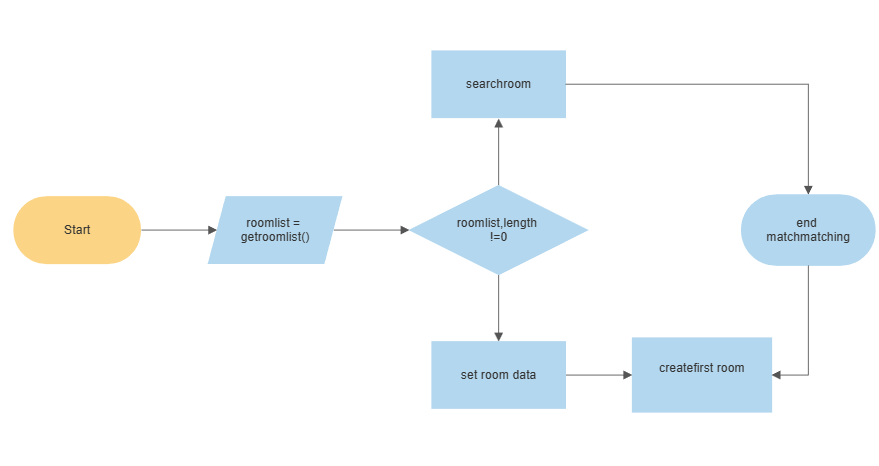
\includegraphics[width=15cm]{flowchart-matchmaking}
%     \label{fig:algoritmamatmaching}
%     \end{figure}


%     Mengacu pada gambar \ref{fig:algoritmamatmaching}, algoritma membutuhkan daftar \textit{room} yang didapatkan dari \textit{interface} photon \textit{Behavior}. Jika belum ada \textit{room} yang tersedia pada daftar \textit{room}, maka dilakukan fungsi detil dari algoritma matchmaking yaitu SearchRoomMatchmaking(). Berikut detil penjelasan flowchart pada gambar \ref{fig:detail-mm-1} dan gambar \ref{fig:detail-mm-2}.
%     \newpage
%     \begin{figure}[h]
%         \centering
%         \caption{Detail Algoritma Matchmaking 1}
%         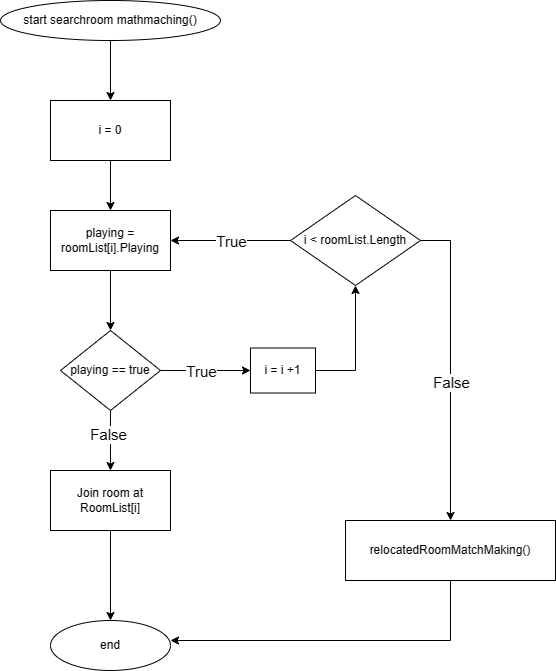
\includegraphics[width=10cm]{detail-algoritma-matmaking1.png}
%         \label{fig:detail-mm-1}
%         \end{figure}


%         Mengacu pada Gambar \ref{fig:detail-mm-1}, ketika fungsi ini dipanggil, 
% maka ia akan memulai perulangan sebanyak daftar room yang 
% tersedia. Pencarian bertujuan untuk mencari room yang memiliki 
% status sedang tidak bermain (waiting). Jika tidak menemukan 
% room yang tersedia dan ber-status tidak sedang bermain (waiting) 
% maka akan dilakukan pemanggilan fungsi 
% RealocateRoomMatchmaking() yang dijelaskan lebih detil pada 
% Gambar \ref{fig:detail-mm-2}. Jika sebaliknya maka pemain akan bergabung ke 
% dalam room.

% \newpage
% \begin{figure}[h]
%     \centering
%     \caption{Detail Algoritma Matchmaking 2}
%     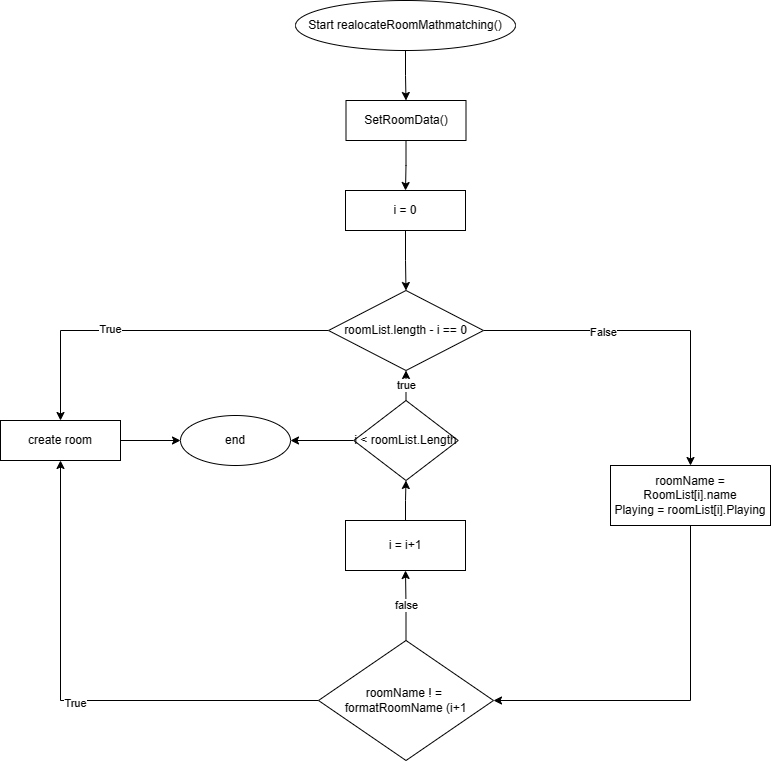
\includegraphics[width=10cm]{detail-algoritma-matmaking2.png}
%     \label{fig:detail-mm-2}
%     \end{figure}

\subsection{Rancangan Use Case Diagram}
\begin{enumerate}
    \item \textit{Use Case Diagram}
    \\ Tahapan ini memiliki satu aktor yaitu pemain, penjelasan mengenai tahap ini diilustrasikan pada gambar \ref{fig:case-diagram}
    \begin{figure}[h]
        \centering
        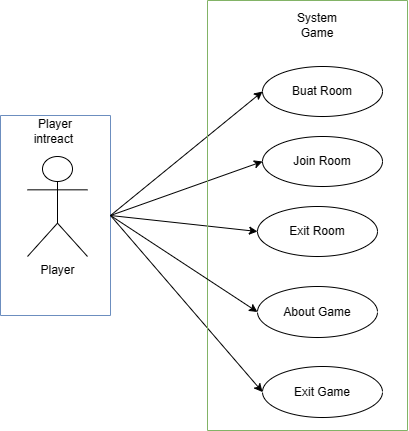
\includegraphics[width=10cm]{case-diagram.png}
        \caption{Use Case Diagram}
        \label{fig:case-diagram}
    \end{figure}

    Gambar \ref{fig:case-diagram} menjelaskan tentang \textit{Use Case Diagram} dimana terdapat satu aktor yaitu pemain, serta 5 \textit{Use Case} yaitu \textit{Buat Room, Join Room, Exit Room, About Game, Exit Game}.
    Pemain dapat menjadi server jika pemain melakukan \textit{use case} buat room dan pemain juga bisa menjadi client jika pemain menggunakan \textit{use case join room}, tetapi jika tidak adanya pemain yang menggunakan \textit{use case} buat room, maka \textit{use case} join room tidak dapat digunakan oleh pemain yang menjadi client.
    \textit{use case exit room} dapat dilakukan oleh pemain yang menjadi server maupun menjadi client, dan hal itu akan menghapus sesi room yang sudah dibuat jika semua pemain menggunakan \textit{use case exit room}. \textit{Use case about game} dapat dilakukan oleh pemain untuk mengetahui tentang \textit{game} yang dimainkan, dan yang terakhir jika pemain ingin meninggalkam \textit{game}, pemain mengunakan \textit{Use case Exit Game.}
    \textit{Activity diagram} adalah diagram yang memodelkan aliran aktivitas pada sistem.
    \item Activity Diagram
    \begin{enumerate}
        \item \textit{Activity Diagram} buat \textit{Room}
        \begin{figure}[h]
           \centering
           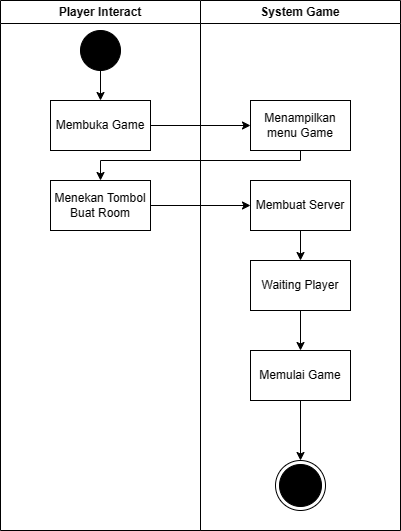
\includegraphics[width=10cm]{room-diagram.png}
           \caption{Activity Diagram Create Room}
           \label{fig:croom-case}
       \end{figure}
       \\ Gambar \ref{fig:croom-case} merupakan \textit{Activity Diagram Create Room}. Diawali dengan pemain membuka \textit{game}, sistem akan menampilkan menu \textit{game}, player menekan tombol buat room untuk membuat room yang belum tersedia sebagai server atau pemilk room.
       Pada \textit{activity waiting player} pemilik room akan menunggu player/\textit{client} untuk memasukan room dan memulai \textit{game}.
       \newpage
    \item \textit{Activty Diagram} join \textit{Room}
    \begin{figure}[h]
        \centering
        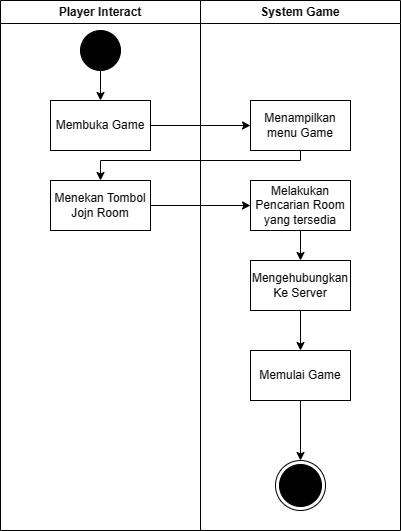
\includegraphics[width=10cm]{joinroom-diagram.png}
        \caption{Activity Diagram Join Room}
        \label{fig:jroom-case}
    \end{figure}
    \\ Gambar \ref{fig:jroom-case} merupakan \textit{activity diagram join room}. Diawali dengan pemain membuka \textit{game}, kemudian sistem akan menampilkan menu dari \textit{game}, player menekan tombol join room, photon unity akan mencarikan room yang tersedia yang sudah dibuat oleh pemain lain atau bisa mengetikan manual custom port yang terdapat pada pembuat room. Pemain akan terhubung ke server atau room yang tersedia jika room valid.
    \newpage
    \item  \textit{Activity Diagram Exit Room}
    \begin{figure}[h]
        \centering
        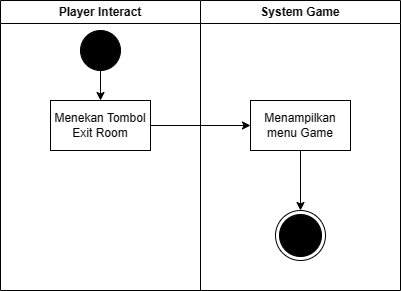
\includegraphics[width=10cm]{exitroom-diagram.png}
        \caption{Activity Diagram Exit Room}
        \label{fig:eroom-case}
    \end{figure}
    \\ Gambar \ref{fig:eroom-case} merupakan \textit{activity diagram exit room}. Diawali dengan pemain menekan tombol exit room, sistem akan menampilkan menu utama pada \textit{game}.    
    \item \textit{Activity Diagram About Room}
     \begin{figure}[h]
        \centering
        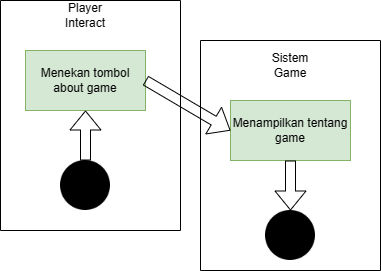
\includegraphics[width=10cm]{aboutcase-diagram.png}
        \caption{Activity Diagram About Room}
        \label{fig:aroom-case}
    \end{figure}
    \\ Gambar \ref{fig:aroom-case} merupakan \textit{activity diagram about room}. Diawali dengan pemain menekan tombol \textit{about room}. Sistem akan menampulkan isi tentang \textit{game} yang dimainkan.
    \item  \textit{Activity Diagram Exit Game}
    \begin{figure}[h]
        \centering
        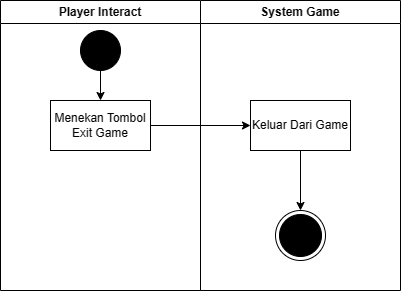
\includegraphics[width=10cm]{exitgame-diagram.png}
        \caption{Activity Diagram Exit \textit{game}}
        \label{fig:egame-case}
    \end{figure}
    \\ Gambar \ref{fig:egame-case} merupakan \textit{activity diagram exit game}. Diawali dengan pemain menekan tombol \textit{exit game}. Sistem akan mengeluarkan pemain dari game yang sedang dimainkan.
\end{enumerate}
\end{enumerate}

    % \item \textit{Activity Player}
    % \begin{figure}[h]
    %     \centering
    %     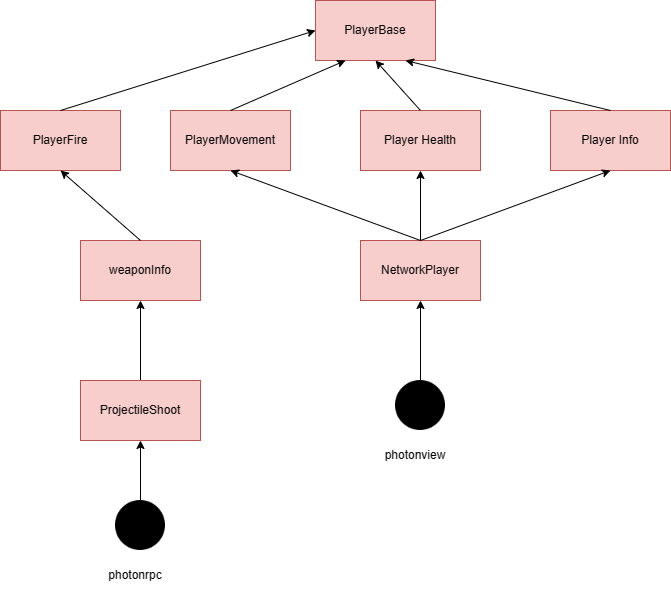
\includegraphics[width=10cm]{player-case.png}
    %     \caption{Activity Diagram Player}
    %     \label{fig:player-case}
    % \end{figure}
    % \\ Gambar \ref{fig:player-case} merupakan \textit{Activity Diagram Player}. Diawali dengan pemain harus terkoneksi jaringan photon, kemudian sistem akan memasuki ke layer network, yang akan menghubungkan beberapa komponen yaitu player movement, player health dan player info.
    % Pada \textit{photon RPC} player memasuki ke sistem sinkronisasi kedalam \textit{projectileshoot} yang berfungsi disini sebagai menambak player musuh, kemudian memasukin activit weapon info yang berisi \textit{ammo weapon}, dan dari ammo yang tersedia mamsuki activity playerfire yang menandakan player siap memerangi player lain.
    % \newpage
    



% \subsection{Rancangan Arsitektur Umum Matchmaking}
% Photon memiliki fitur dan metode sendiri dalam mengelola sebuah \textit{game} multiplayer yang menggunakan \textit{framework}-nya.
% Photon Unity Networking merupakan class library yang dibungkus menjadi framework untuk mengelola pertukaran data sinkronisasi antar klien melalui Photon Cloud. 
% Arsitektur aplikasi permainan jak meuprang ini pada umumnya mempertemukan player pada lobby terlebih dahulu sebagai syarat memulai permainan dengan memanfaatkan event dan state yang ada pada Photon Unity Networking, komponen data pemain dan \textit{room} tersimpan dalam \textit{Custom Properties}. Berikut adalah arsitektur sistem dari aplikasi permainan pada Gambar \ref{fig:rumum-arsi}.
% \newpage
% \begin{figure}
%     \centering
%     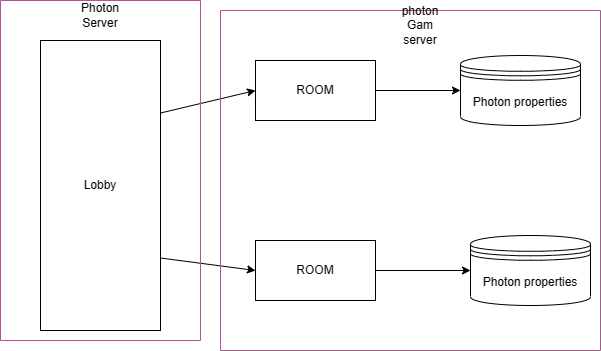
\includegraphics[width=10cm]{rancangan-arsitektur.png}
%     \caption{Rancangan Arsitektur Umum Matchmaking}
%     \label{fig:rumum-arsi}
% \end{figure}

% \subsection{Class Diagram Network}
% \noindent

% Rancangan kelas diagram ini merupakan bagian penting dari fitur \textit{Synchronous Multiplayer} dan akan diimplementasikan sesuai dengan rancangan diagram kelas seperti gambar \ref{fig:class-network}.

% Pada kelas NetworkSpawner berfungsi untuk melakukan instansiasi objek karakter pemain dan menghidupkan kembali jika karakter pemain dalam keadaan \textit{state} mati.

% Pada kelas NetworkMatchmaking, kelas ini akan menunggu event dari kelas NetworkManager. NetworkMatchmaking tidak dapat berjalan tanpa dikendalikan oleh NetworkManager.

% Photon memiliki fitur penyimpanan \textit{state} sementara pada \textit{server}-nya (Photon Cloud), fitur tersebut berguna untuk menyimpan informasi \textit{room}, skor \textit{leaderboard} tiap pemain.
% Fiture tersebut yaitu Photon Room Properties dan Photon Player Properties.
% Perbedaanya adalah, penyimpanan dalam Photon Room Properties dapat diketahui nilainya oleh klien dalam satu \textit{room} yang sama, tetapi jika ingin mendapatkan nilai informasi dalam sebuah \textit{room} melalui Photon Room Properties, maka \textit{masterclient} diroom yang bersangkutan harus melakukan pengaturan pada \textit{method} CustomPropertiesForLobby yang terdapat pada photon.
% Sedangkan Photon Player Properties hanya dapat diakses ketika dalam satu room yang sama.

% NetworkPlayerProperty dan NetworkRoomProperty bertugas untuk menyimpan nilai \textit{unique} yang terdapat pada Photon Player Properties dan Photon Room Properties.

% \begin{figure}[h]
%     \centering
%     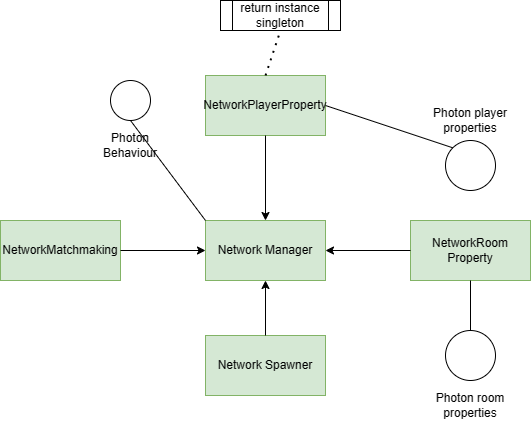
\includegraphics[width=8cm]{class-diagram-network.png}
%     \caption{Class Diagram Network}
%     \label{fig:class-network}
% \end{figure}

% \begin{enumerate}
%     \item Activity Class Diagram Network
%     \begin{figure}[h]
%         \centering
%         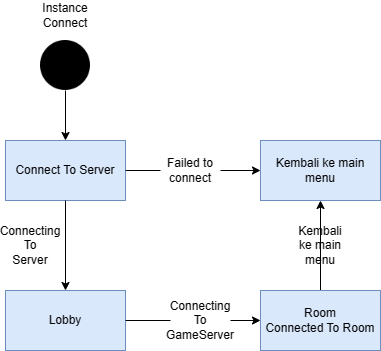
\includegraphics[width=8cm]{activity-class-network.png}
%         \caption{\textit{Activity Class Diagram Network}}
%         \label{fig:activity-class-network}
%     \end{figure}
%     \newpage
%     Dapat dilihat pada gambar \ref{fig:activity-class-network} digambarkan alur kerja atau aktivitas sebuah system \textit{photon unity networking} yang dimulai dengan terkoneksi internet kemudian sistem akan melakukan koneksi ke \textit{photon}. Jika gagal menghubungkan maka sistem akan mengembalikan pemain ke layar menu, jika berhasil player akan memasuki lobby.
%     Pada saat dilobby pemain akan memasuki kondisi kedua, menghubungkan pemain ke dalam game server, jika sudah ter-\textit{connect} maka pemain akan memasuki \textit{room} yang sudah dihubungkan. Jika semua activity sudah dilakukan dan pemain sudah menghabiskan pada \textit{room} terssebut maka pemain akan dikembalikan ke main menu.
% \end{enumerate}

\subsection{Rancangan \textit{Class Diagram Multiplayer}}
\begin{figure}[h]
   \centering
   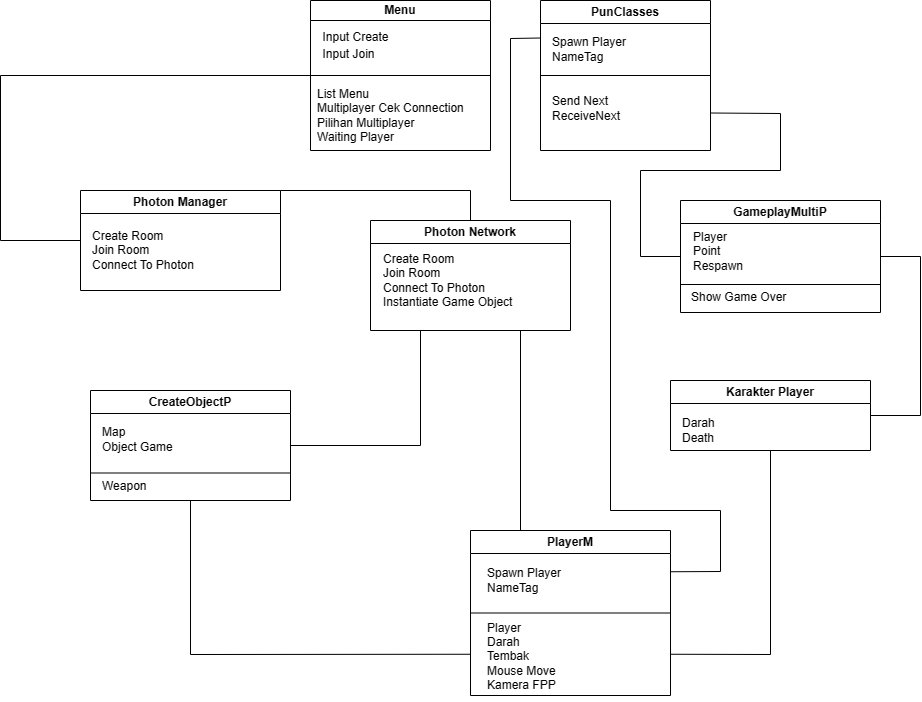
\includegraphics[width=10cm]{class-diagram-perancangan.png}
    \caption{Rancangan \textit{class diagram} multiplayer}
    \label{fig:class-diagram-game}
\end{figure}

Pada gambar \ref{fig:class-diagram-game} merupakan perancangan sistem multiplayer yang akan diterapkan pada gim.
Class PhotonNetwork dan PunClasses merupakan class yang ada pada library photon.
Class PhotonManager merupakan class yang menampung fungsi untuk menyambungkan ke server, membuat \textit{room} dan bergabung pada \textit{room} yang ada.
Class menu sendiri berfungsi sebagai \textit{interface} pada main menu gim, semua aksi yang ada pada main menu ditampung pada class menu.
CreateObjectP merupakan kelas yang berfungsi untuk membuat map atau \textit{game} object yang diinisialisasi.
PlayerM merupakan kelas yang berfungsi untuk menampung semua pergerakan player seperti pergerakan,darah,menembak, dan kamera.
GameplayMultiP merupakan class yang berfungsi sebagai \textit{gameplay} yang akan dimainkan seperti player, point pada \textit{game} dan respawn pemain saat mati.
Dan KarakterPlayer merupakan class yang berfungsi sebagai inisialisasi player utama.
\begin{enumerate}
    \item Blok \textit{Diagram Gameplay}
    \begin{figure}[h]
        \centering
        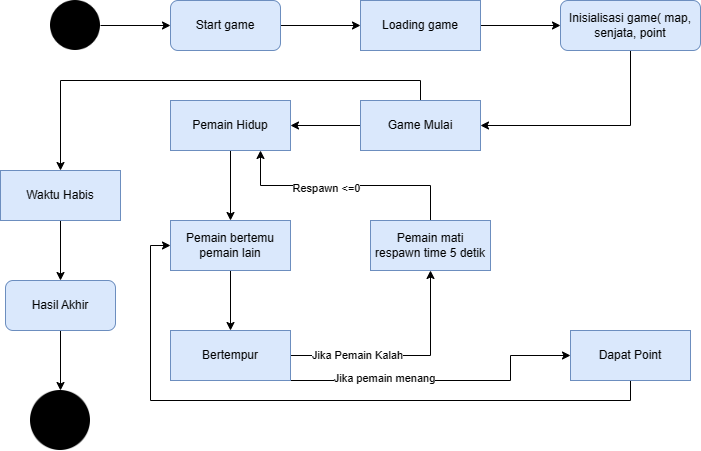
\includegraphics[width=10cm]{blok-diagram-game.png}
        \caption{\textit{Blok Diagram Gameplay}}
        \label{fig:aclass-diagram-game}
    \end{figure}

    Dapat dilihat pada gambar \ref{fig:aclass-diagram-game} digambarkan alur kerja atau aktivitas sebuah sistem \textit{game} yang dimulai \textit{start game} untuk memulai permainan kemudian menunggu \textit{loading} untuk memasuki permainan, sistem akan menginisialisasi objectnya terlebih dahulu seperti map, senjata dan point.
    Jika inisialisasi sudah selesai \textit{game} akan dimulai dan pemain spawn pada saat \textit{game} dimulai, jika pemain bertemu pemain lain dan bertempur akan ditemukan dua kondisi, jika mati pemain akan \textit{respawn} ulang dengan waktu 5 detik, jika pemain memenangkan pertempuran maka pemain mendapatkan point.
    Ketika \textit{game} sudah habis waktu makan \textit{game} sudah berakhir dan akan mamasukin akhir \textit{game} permainan.
\end{enumerate}
\newpage
\subsection{Alur Diagram Monitoring}
\begin{figure}[h]
    \centering
    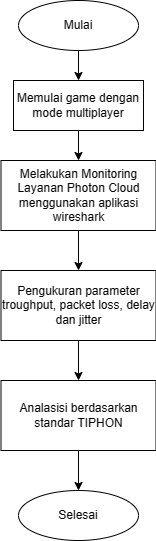
\includegraphics[width=3cm]{alur-diagram-monitoring.png}
    \caption{Alur Diagram Monitoring}
    \label{fig:alur-diagram}
\end{figure}

Dapat dilihat pada gambar \ref{fig:alur-diagram} digambarkan alur diagram monitoring jaringan dengan menggunakan wireshark qos, untuk mengetahui performa dari photon cloud yang disediakan oleh unity.
Pada langkah pertama akan dimulai game terlebih dahulu dengan mode multiplayer online, kemudian melakukan monitoring photon cloud menggunakan aplikasi wireshark, kemudian diukurkan parameter \textit{troughput, packet loss, delay} dan \textit{jitter} dengan memasuki 2-3 player.
Kemudian dianalisis berdasrkan standar TIPHON.
\newpage
\section{Metode Penelitian}
\noindent

Photon memiliki fitur dan metode sendiri dalam mengelola sebuah \textit{game} multiplayer yang menggunakan \textit{framework}-nya. Untuk mengelola metode yang telah disediakan oleh photon, peniliti mengimplementasikan metode matchmaking pada \textit{game} \textit{multiplayer first person shooter}(fps) untuk mencari roomlist atau create room pada \textit{game} \textit{first person shooter}.
        \begin{figure}[h]
         \centering
         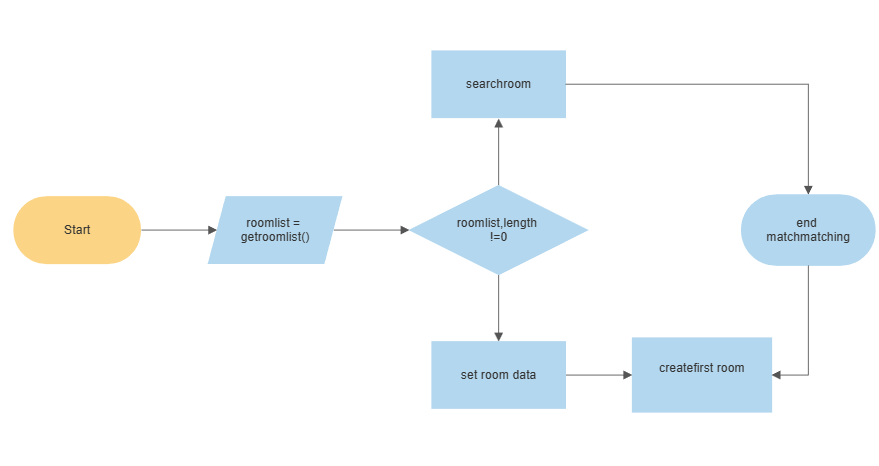
\includegraphics[width=10cm]{flowchart-matchmaking}
         \caption{Flowchart Algoritma Matchmaking}
         \label{fig:algoritmamatmaching}
         \end{figure}

Mengacu pada gambar \ref{fig:algoritmamatmaching}, algoritma membutuhkan daftar \textit{room} yang didapatkan dari \textit{interface} photon \textit{Behavior}. Jika belum ada \textit{room} yang tersedia pada daftar \textit{room}, maka dilakukan fungsi detil dari algoritma matchmaking yaitu SearchRoomMatchmaking(). 

% Berikut detil penjelasan flowchart pada gambar \ref{fig:detail-mm-1} dan gambar \ref{fig:detail-mm-2}.
% \begin{figure}[h]
%             \centering
%             \caption{Detail Algoritma Matchmaking 1}
%             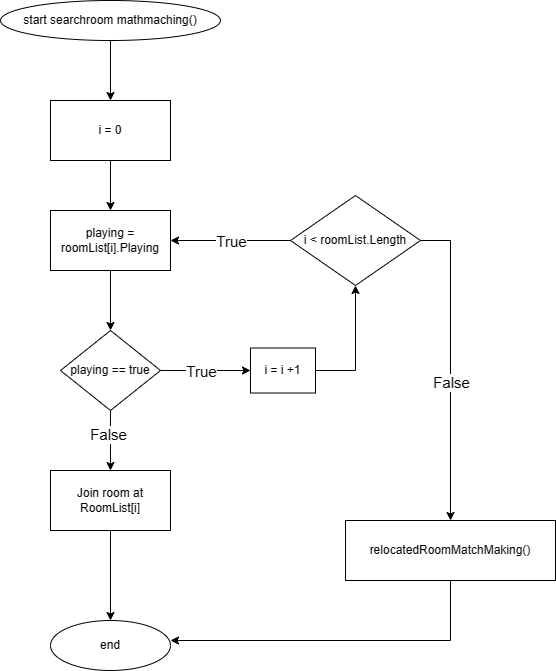
\includegraphics[width=10cm]{detail-algoritma-matmaking1.png}
%             \label{fig:detail-mm-1}
%             \end{figure}
    
    
%             Mengacu pada Gambar \ref{fig:detail-mm-1}, ketika fungsi ini dipanggil, 
%     maka ia akan memulai perulangan sebanyak daftar room yang 
%     tersedia. Pencarian bertujuan untuk mencari room yang memiliki 
%     status sedang tidak bermain (waiting). Jika tidak menemukan 
%     room yang tersedia dan ber-status tidak sedang bermain (waiting) 
%     maka akan dilakukan pemanggilan fungsi 
%     RealocateRoomMatchmaking() yang dijelaskan lebih detil pada 
%     Gambar \ref{fig:detail-mm-2}. Jika sebaliknya maka pemain akan bergabung ke 
%     dalam room.
    
%     \newpage
%     \begin{figure}[h]
%         \centering
%         \caption{Detail Algoritma Matchmaking 2}
%         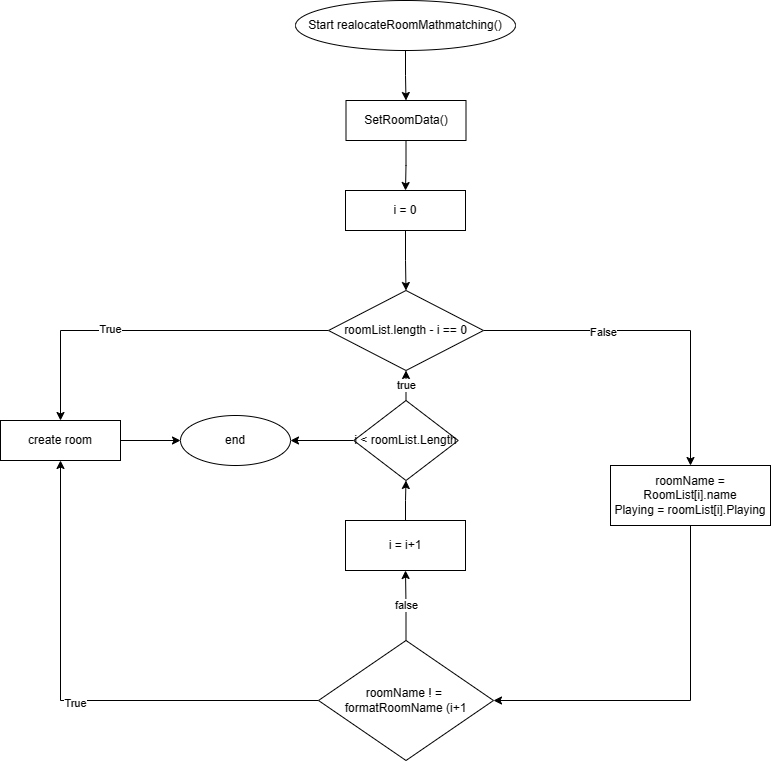
\includegraphics[width=10cm]{detail-algoritma-matmaking2.png}
%         \label{fig:detail-mm-2}
%         \end{figure}

        \section{Teknik Pengujian}
        \subsection{Blackbox}
Teknik pengujian yang digunakan yaitu blackbox. Pengujian Black Box pada fungsional sistem yang terdapat pada aplikasi permainan \textit{first person shooter}.

    \begin{table}[h]
    \centering
    \caption{Tabel Pengujian Black Box}
    \label{lab:tabel-pengujian}
    \begin{tabular}{|l|l|l|l|}
    \hline
    \multicolumn{1}{|c|}{NO} & \multicolumn{1}{c|}{Aktivitas Pengujian} & \multicolumn{1}{c|}{Hasil yang diharapkan} & \multicolumn{1}{c|}{Kesimpulan} \\ \hline
    1                        & Tombol Buat Room                         & Membuka panel "Room Panel"                 &                                 \\ \hline
    2                        & Tombol Join Room                         & Membuka panel "Lobby Panel"                &                                 \\ \hline
    3                        & Tombol Exit Room                         & Kembali ke menu utama                      &                                 \\ \hline
    4                        & Tombol About Game                        & Menampilkan popup about game               &                                 \\ \hline
    5                        & Tombol exit game                         & Keluar dari aplikasi game                  &                                 \\ \hline
    \end{tabular}
    \end{table}
\newpage        
\subsection{Pengujian performa jaringan}
Teknik pengujian performa untuk melakukan pengujian jaringan pada photon cloud menggunakan wireshark qos untuk mengukur troughput, delay dan packet loss.
\section{Hasil yang diharapkan}
Hasil yang diharapkan pada penilitian ini antara lain :
\begin{enumerate}
    \item Keberhasilan dalam mengetahui kelayakan aplikasi \textit{game} dengan metode \textit{blackbox testing}, dan pengujian performa jaringan.
    \item Keberhasilan \textit{game} terhubung dengan unity python networking yang dapat dimainkan secara multiplayer online.
    \item Laporan tugas akhir mahasiswa jurusan Teknologi Informasi Dan Komputer.
\end{enumerate}
\chapter*{JADWAL KEGIATAN PENELITIAN}
\addcontentsline{toc}{chapter}{JADWAL KEGIATAN PENELITIAN}
Berikut jadwal kegiatan yang sudah disiapkan untuk menyiapkan skripsi.


\begin{table}[!ht]
\caption{Jadwal Kegiatan}
\label{tab:jadwal-kegiatan}
\begin{tabular}{|c|m{5cm}|p{.2cm}|p{.2cm}|p{.2cm}|p{.2cm}|p{.2cm}|p{.2cm}|p{.2cm}|p{.2cm}|p{.2cm}|p{.2cm}|p{.2cm}|p{.2cm}|}
\hline
\multirow{2}{*}{No}	& 
\multicolumn{1}{c|}{\multirow{2}{*}{Kegiatan}}	& 
\multicolumn{4}{c|}{Mar} & 
\multicolumn{4}{c|}{Apr} &
\multicolumn{4}{c|}{Mei} \\ \cline{3-14}
& & 
\multicolumn{1}{c|}{1} &
\multicolumn{1}{c|}{2} &
\multicolumn{1}{c|}{3} &
\multicolumn{1}{c|}{4} &
\multicolumn{1}{c|}{1} &
\multicolumn{1}{c|}{2} &
\multicolumn{1}{c|}{3} &
\multicolumn{1}{c|}{4} &
\multicolumn{1}{c|}{1} &
\multicolumn{1}{c|}{2} &
\multicolumn{1}{c|}{3} &
\multicolumn{1}{c|}{4} \\ \hline
1  & Pengumpulan Data 			& \cellcolor{gray!75} & \cellcolor{gray!75} & & & & & & & & & & \\ \hline
2  & Identifikasi Masalah 		& & & \cellcolor{gray!75} & & & & & & & & & \\ \hline
3  & Analisis Kebutuhan Sistem 	& & \cellcolor{gray!75} & \cellcolor{gray!75} & \cellcolor{gray!75} & & & & & & & & \\ \hline
4  & Membuat Rancangan Sistem 	& & & & \cellcolor{gray!75} & \cellcolor{gray!75} & & & & & & & \\ \hline
5  & Rancang Bangun Program 	& & & & & & \cellcolor{gray!75} & \cellcolor{gray!75} & \cellcolor{gray!75} & & & & \\ \hline
6  & Uji coba program (\textit{testing}) 			& & & & & & & & \cellcolor{gray!75} & \cellcolor{gray!75} & & & \\ \hline
7  & Revisi Konsep, Desain Rancangan, Code Program & & & & & & & & & \cellcolor{gray!75} & \cellcolor{gray!75} & & \\ \hline
8  & Implementasi Program 					& & & & & & & & & & & \cellcolor{gray!75} & \\ \hline
9  & Pembimbingan Penulisan Naskah Skripsi & & & & & \cellcolor{gray!75} & \cellcolor{gray!75} & \cellcolor{gray!75} & \cellcolor{gray!75} & \cellcolor{gray!75} & & & \\ \hline
10 & Penulisan Akhir Laporan 				& & & & & & & & & & \cellcolor{gray!75} & & \\ \hline
11 & Pendanaan							& & & & & & & & & & & & \cellcolor{gray!75} \\ \hline
\end{tabular}
\end{table}


\chapter*{RENCANA ANGGARAN PENELITIAN}
\addcontentsline{toc}{chapter}{RENCANA ANGGARAN PENELITIAN}
Rencana anggaran penelitian pada pembuatan penelitian “Rancang Bangun Game Mulitplayer Online First Person Shooter(FPS) 3D Menggunakan Photon Unity Networking”.

\begin{table}[h]
    \centering
    \begin{tabular}{|llcl|l|ll}
    \cline{1-5}
    \multicolumn{1}{|c|}{NO} & \multicolumn{1}{c|}{Uraian}          & \multicolumn{1}{c|}{Volume}  & \multicolumn{1}{c|}{Harga(Rp)} & Jumlah(Rp)    &  &  \\ \cline{1-5}
    \multicolumn{1}{|l|}{1}  & \multicolumn{1}{l|}{Kuota}           & \multicolumn{1}{c|}{3 Bulan} & Rp.90.000                      & Rp. 180.000   &  &  \\ \cline{1-5}
    \multicolumn{1}{|l|}{2}  & \multicolumn{1}{l|}{Kertas hvs a4}           & \multicolumn{1}{c|}{5 rim} & Rp.200.000                      & Rp. 200.000   &  &  \\ \cline{1-5}
    \multicolumn{4}{|c|}{Jumlah}                                                                                                    & Rp. 180.000 &  &  \\ \cline{1-5}
    \end{tabular}
    \caption{Anggaran Penelitian}
    \label{lab:label-anggaran}
    \end{table}

\begin{thebibliography}{9}
\bibitem{Sarwodi}
Sarwodi, S.S., Wardhono, W.S. and Akbar, M.A., 2020. \emph{Penerapan Multiplayer Pada Gim Tower Defense Menggunakan Photon Unity.}, Jurnal Pengembangan Teknologi Informasi dan Ilmu Komputer e-ISSN, 2548, p.964X.

\bibitem{Ansori}
Pratama, R.N., Ansori, A.S.R. and Dinimaharawati, A., 2021 \emph{Pembuatan Multiplayer Game Ucing Beling Menggunakan Asset Store Mirror}, eProceedings of Engineering, 8(5).
Wesley, Massachusetts, 2nd ed.

\bibitem{fps}
Ramadhan, I. and Purwanto, A., 2020. \emph{Pengembangan Teknologi Game Indonesia Untuk Permainan First Person Shooter (Fps) 3d Multiplayer “Code To Shoot” Menggunakan Unity Network (Unet) Berbasis Mobile.} Jurnal Teknologi Informasi Universitas Lambung Mangkurat (JTIULM), 5(2), pp.39-48.

\bibitem{fps2013}
Halim, M., 2013. \emph{PEMBUATAN GAME “THE LAST MISSION” DENGAN MENGGUNAKAN FPS CREATOR} (Doctoral dissertation, Universitas AMIKOM Yogyakarta).

\bibitem{androidsdk}
Download Android Studio and SDK Tools | Android 
Developers," Google, [Online]. Available: 
http://developer.android.com/sdk/index.html. [Accessed 08 
Maret 2023].

\bibitem{pun}
Photon Unity Networking 2," Unity, 
[Online]. Available : https://doc-api.photonengine.com/en/pun/v2/. [Accessed 08 Maret 2023]

\bibitem{Gebug}
Suartama, I., 2020. \emph{Pengembangan Game Multiplayer Pengenalan Budaya Gebug Ende Seraya Karangasem Berbasis Android} (Doctoral dissertation, Universitas Pendidikan Ganesha).

\bibitem{gogreen}
Fathurrohman, M.F., 2018. \emph{Pembangunan Game Multiplayer Edukasi Go Green 3D Berbasis Android} (Doctoral dissertation, Universitas Komputer Indonesia).
\end{thebibliography}
\addcontentsline{toc}{chapter}{DAFTAR PUSTAKA}

\end{document}
